\subsubsection{Evolution}
In order to allow a decentralized evolution of the system, Goalp do not rely on a centralized model created at design-time. Instead, metadata present into artifacts contained into an artifact repository is used. This allows third party developers to provide software components with different restrictions of the original developer, creating more variability and in consequence, allowing the application to be executed in a more broad range of devices.

evolve without great effort.

We argue that a goal model can be seen as a protocol definition. When we create OR-Refinements we are giving alternatives of execution, creating variability points.

By creating interfaces in variability points
Open deployment platform.

  and we create opportunity for thirty-parties provide new alternativies

having different context condition will allow the goal to be achievable in a broader range of contexts: for example, in screen controls will allow the game to be playable at touch screen devices.

In tradition deployment schema, a complete new version of the software should be released.

\begin{figure}[!htb]
  \centering
  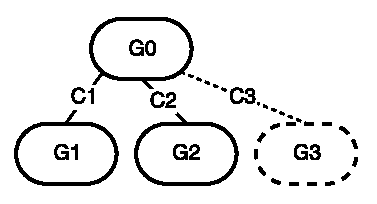
\includegraphics[width=\linewidth]{evolution_or}
  \caption{Evolution OR}
\label{fig:evolution_or}
\end{figure}

Component development and release
